\begin{titlepage}
\begin{center}

% Upper part of the page. The '~' is needed because \\
% only works if a paragraph has started.
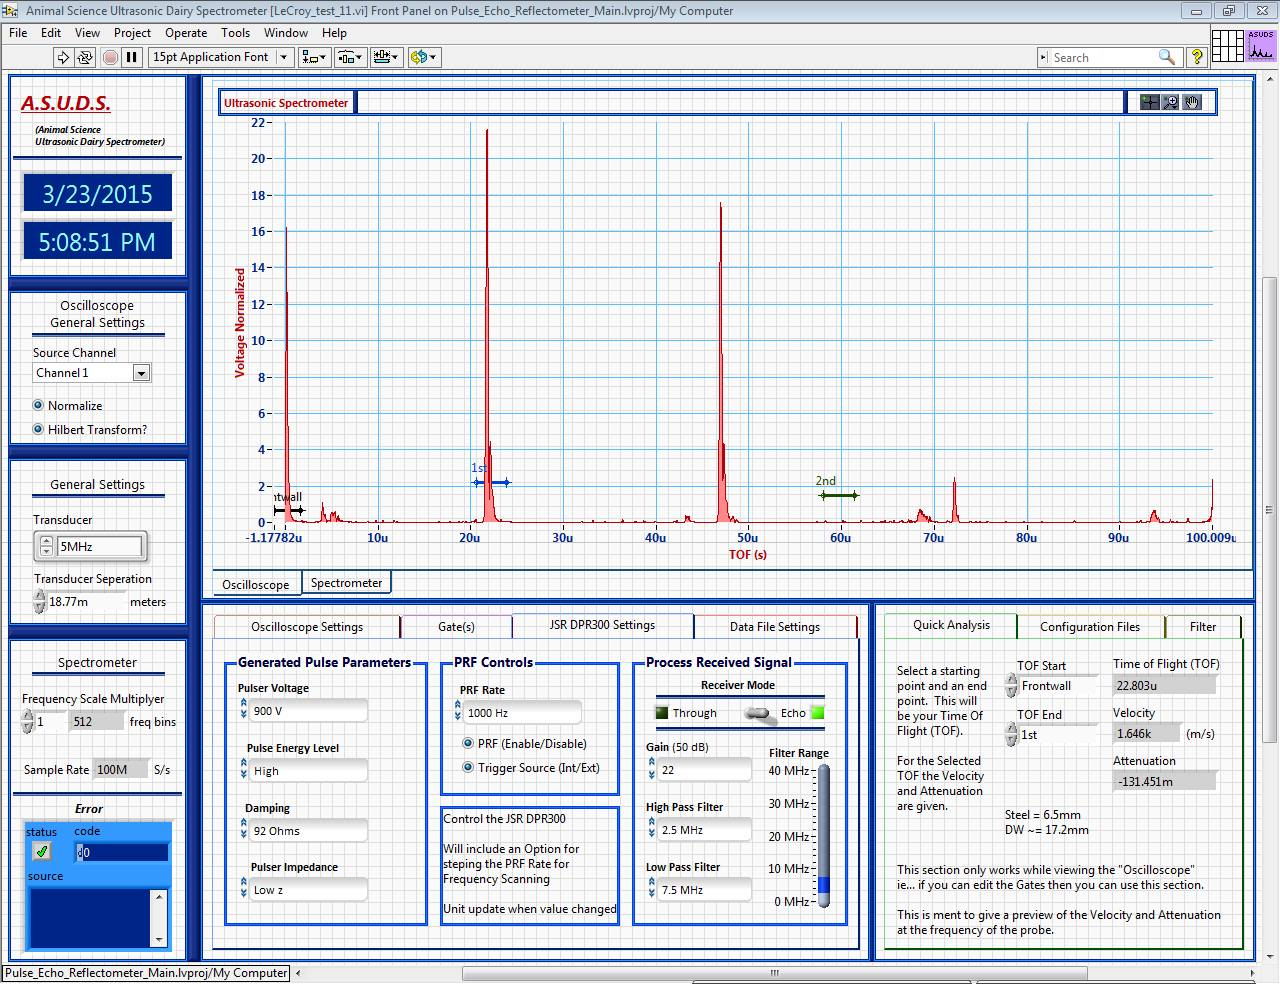
\includegraphics[width=0.15\textwidth]{./title_page}~\\[1cm]

\textsc{\LARGE Ultrasonics Spectrometer Code Manual}\\[1.5cm]

\textsc{\Large Final year project}\\[0.5cm]

% Title
\HRule \\[0.4cm]
{ \huge \bfseries Lager brewing techniques \\[0.4cm] }

\HRule \\[1.5cm]

% Author and supervisor
\noindent
\begin{minipage}[t]{0.4\textwidth}
\begin{flushleft} \large
\emph{Author:}\\
Matthew \textsc{Rothfuss}
\end{flushleft}
\end{minipage}%
\begin{minipage}[t]{0.4\textwidth}
\begin{flushright} \large
\emph{Developer:} \\
Matthew \textsc{Rothfuss}
\end{flushright}
\end{minipage}

\vfill

% Bottom of the page
{\large \today}

\end{center}
\end{titlepage}